% 98-55(98쪽) — 사각형 ABCD($\seg{AB}=7$ · $\seg{BC}=3$ · $\seg{CD}=4$ · $\seg{DA}=6$ · $C=90^\circ$). 스캔 화질이 낮아 TikZ 로 다시 그림.
% 라벨은 원문 것만: 꼭짓점 A·B·C·D, 길이 6·4·3·7 과 C 의 직각 표시. 넓이(답)는 적지 않는다.
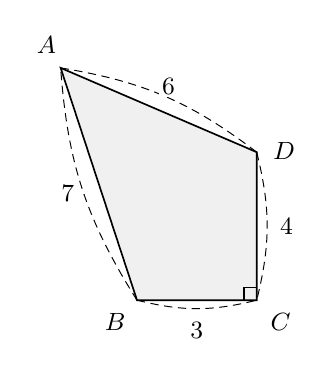
\begin{tikzpicture}[line width=0.6pt, x=1cm, y=1cm]
  \coordinate (A) at (-0.97,2.95);
  \coordinate (B) at (0,0);
  \coordinate (C) at (1.52,0);
  \coordinate (D) at (1.52,1.88);
  \fill[black!6] (A) -- (B) -- (C) -- (D) -- cycle;
  \draw (A) -- (B) -- (C) -- (D) -- cycle;
  % 직각 표시
  \draw[line width=0.45pt] (1.36,0) -- (1.36,0.16) -- (1.52,0.16);
  % 길이 표시의 점선 호
  \draw[densely dashed, line width=0.35pt] (A) to[bend left=14] (D);
  \draw[densely dashed, line width=0.35pt] (D) to[bend left=14] (C);
  \draw[densely dashed, line width=0.35pt] (B) to[bend right=14] (C);
  \draw[densely dashed, line width=0.35pt] (B) to[bend left=14] (A);
  \node[font=\small, fill=white, inner sep=1pt] at (0.40,2.72) {$6$};
  \node[font=\small] at (1.90,0.94) {$4$};
  \node[font=\small] at (0.76,-0.38) {$3$};
  \node[font=\small, fill=white, inner sep=1pt] at (-0.88,1.36) {$7$};
  \node[font=\small, anchor=south east] at (-0.90,3.00) {$\pt{A}$};
  \node[font=\small, anchor=north east] at (-0.02,-0.04) {$\pt{B}$};
  \node[font=\small, anchor=north west] at (1.57,-0.04) {$\pt{C}$};
  \node[font=\small, anchor=west] at (1.60,1.90) {$\pt{D}$};
\end{tikzpicture}
